\documentclass[graphics]{beamer}

\usepackage{graphicx}
\usepackage{verbatim}
\usepackage{wrapfig}
\useoutertheme{shadow}
%\usecolortheme{orchid}
\usecolortheme{seahorse}


% math commands
\newcommand{\be}{\begin{eqnarray}}
\newcommand{\ee}{\end{eqnarray}}
\newcommand{\beq}{\begin{equation}}
\newcommand{\eeq}{\end{equation}}
\def\simless{\mathbin{\lower 3pt\hbox
      {$\rlap{\raise 5pt\hbox{$\char'074$}}\mathchar"7218$}}}
\def\simgreat{\mathbin{\lower 3pt\hbox
      {$\rlap{\raise 5pt\hbox{$\char'076$}}\mathchar"7218$}}} %> or of order

% variables

\def\toonscale{0.45}
\def\mboxy#1{\mbox{\small #1}}


\begin{comment}
\AtBeginSection[]{
  \frame{
    \frametitle{Outline}
    \tableofcontents[currentsection]
  }
}
\end{comment}

\title{Pulsar/FRB VLBI: imaging the highest intensity sources
}
%\subtitle{interim update}
\author[U. Pen]{Ue-Li Pen and collaborators
}
\date{November 3, 2023}


\begin{document}

%\section*{Introduction}
\section{Lenses}

\begin{comment}
  \subsection{Outline}

  \frame{
    \frametitle{Outline}
    \tableofcontents
  }
\end{comment}

\frame{\maketitle}




  \frame{
    \frametitle{Coherent sources: Pulsars, FRBs}
    \begin{itemize}
        \item Coherent, distant source of radiation, highest known
          brightness temperature
        \item Scintillate under multi-path propagation          
        \item sensitive to ns time delay propagating for gigaparsecs
    \end{itemize}
  }


  \frame{

    \frametitle{PSR B0834+06: Coherent VLBI}
\vspace{-0.25in}
\begin{center}
\hspace{-0.5in}
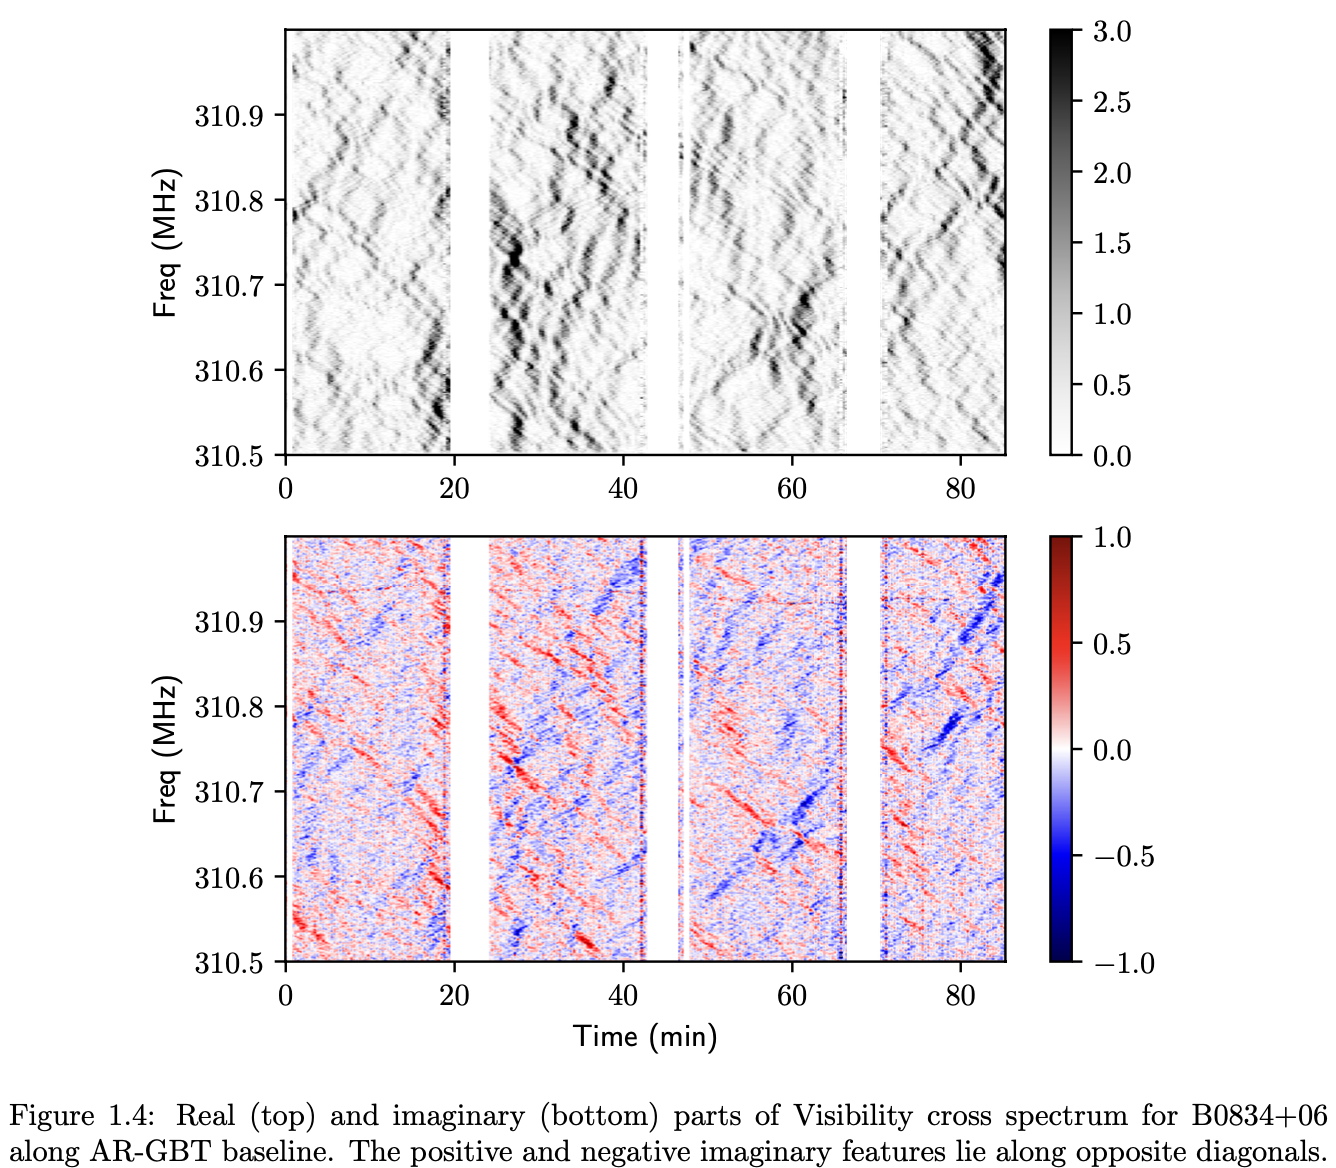
\includegraphics[width=3.5in]{Figures/rawvlbi.png}
\end{center}
  }
  \frame{
%\vspace{-0.25in}
    \frametitle{Scintillometry VLBI}
\hspace{-0.25in}
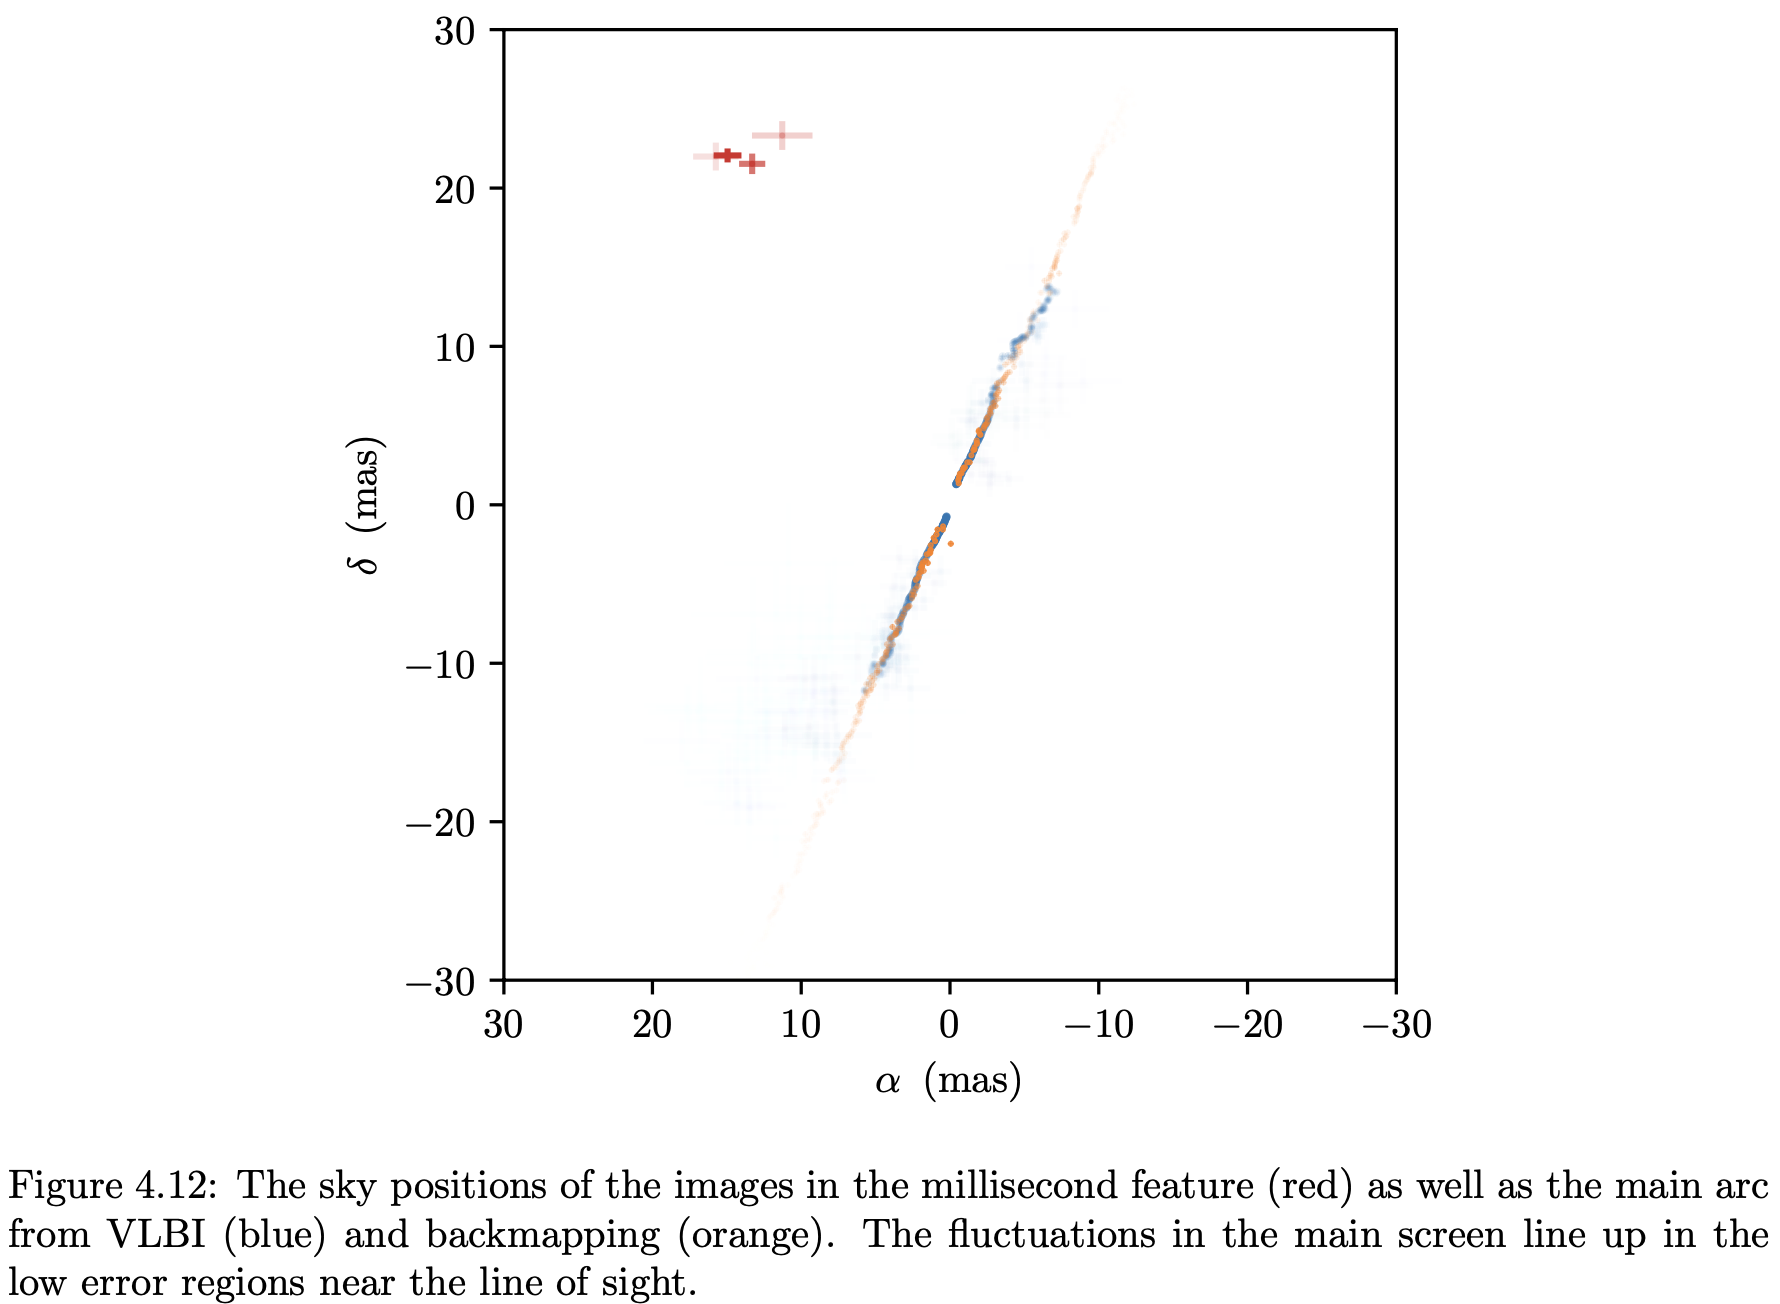
\includegraphics[width=3.5in]{Figures/VLBI0834.png}
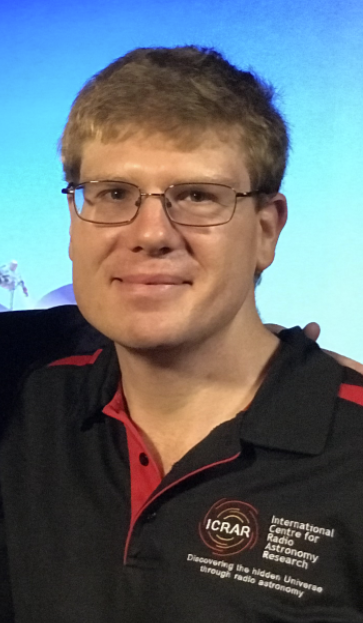
\includegraphics[width=1.05in]{Figures/jpm.png}

Baker++: increase PTA angular resolution to arcminutes.  In memoriam J-P Macquart.
  }


  \frame{

    \frametitle{precision astrometry}
\vspace{-0.25in}
\begin{center}
\hspace{-0.5in}
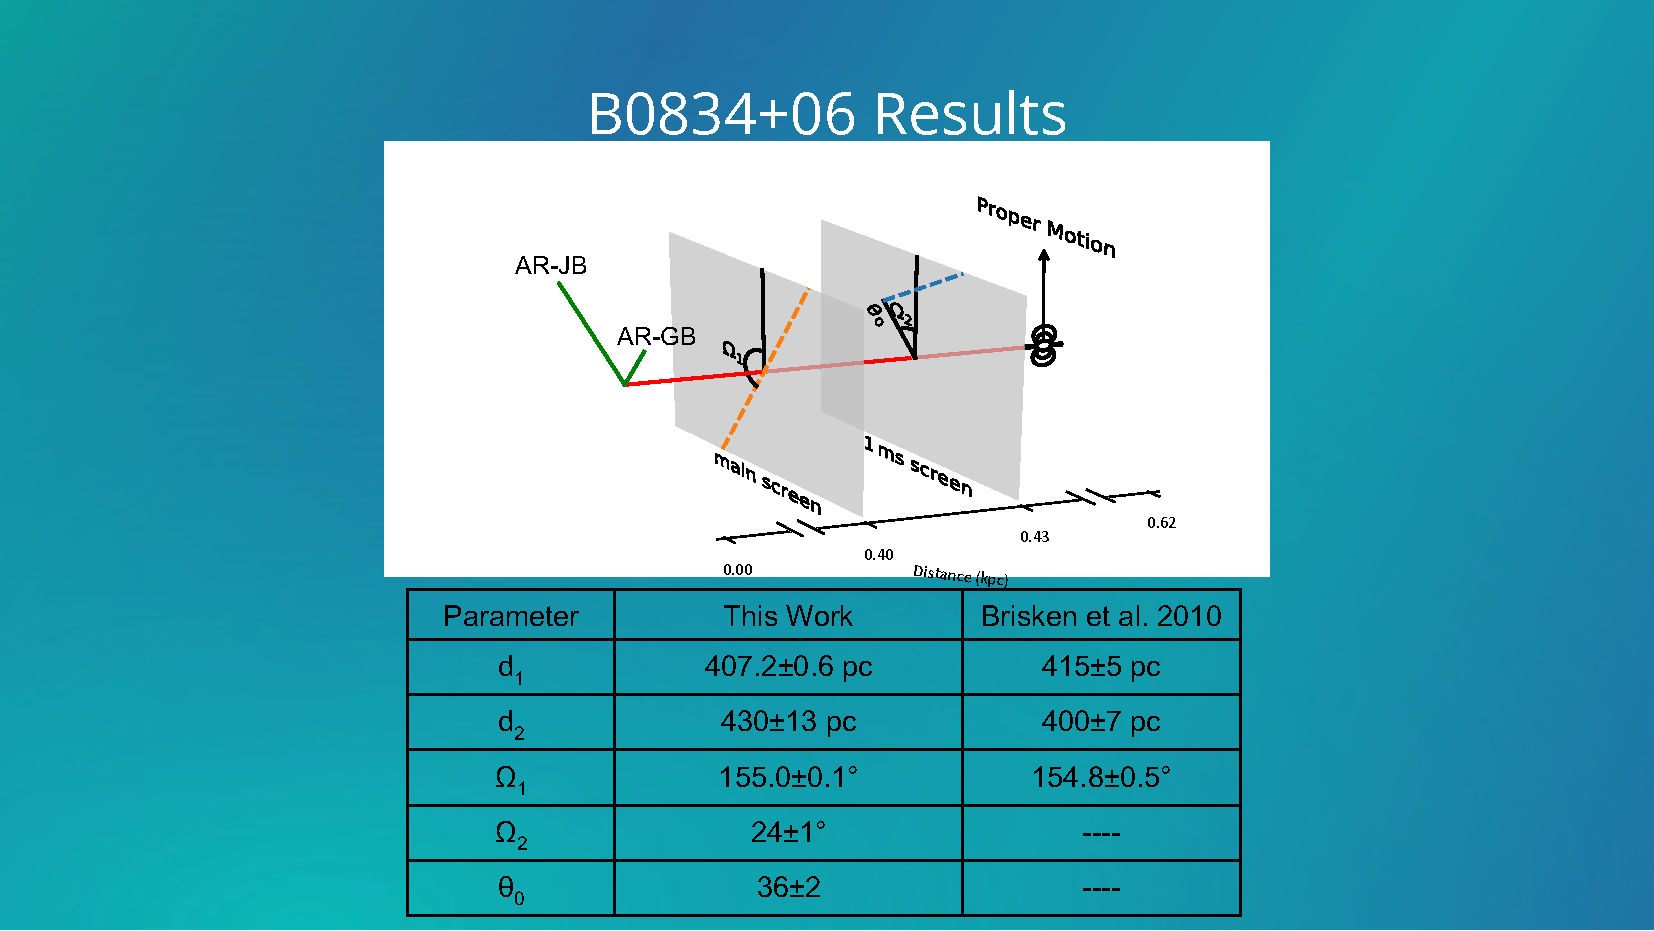
\includegraphics[width=5.5in]{Figures/VLBIdist.pdf}
\end{center}
  }


  \frame{

    \frametitle{more precision astrometry}
%\vspace{-0.25in}
\begin{center}
%\hspace{-0.5in}
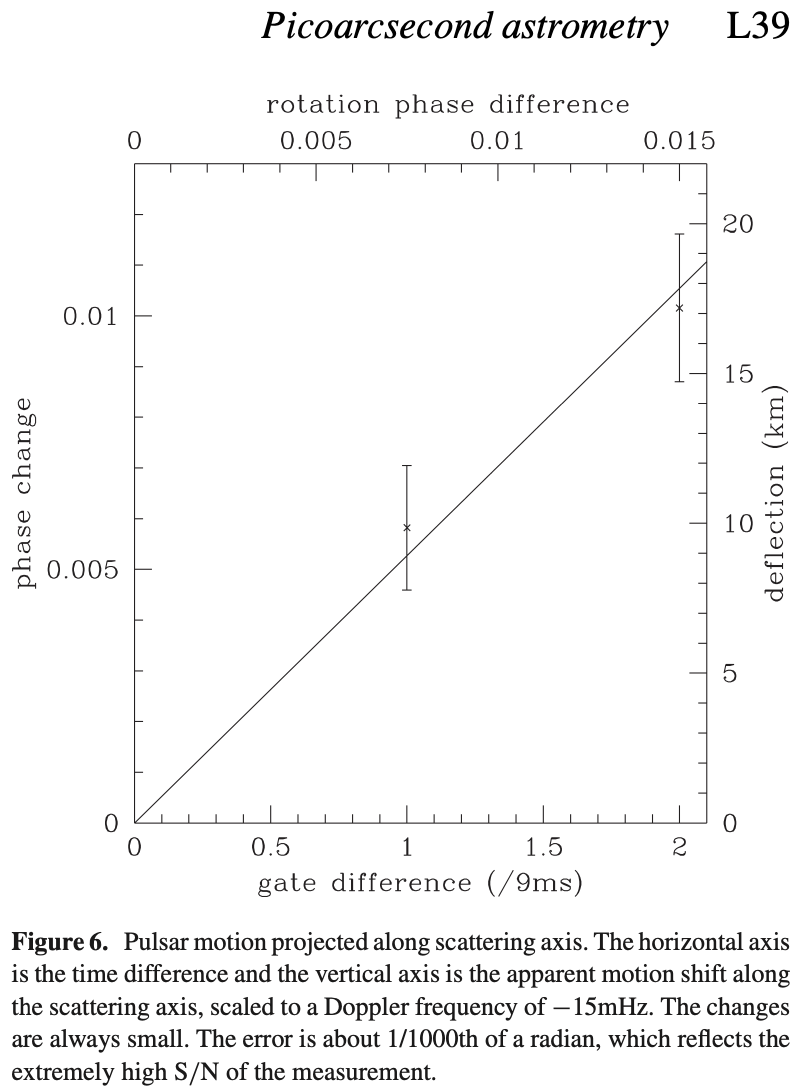
\includegraphics[width=2.05in]{Figures/pico.png}
UP+14
\end{center}
  }





  \frame{
\vspace{-0.5in}
    \frametitle{New Observables}
    \begin{itemize}
    \item for coherent sources: FRBs, pulsars
    \item weak lensing: imaginary image allows time delay measurement (Jow+21)
    \item strong lensing: delay measurements enable measurement of
      co-linearity (Jow++21)
    \item microlensing: instant time delay, planets (Jow+20)
    \item macrolensing: potentially nano-second delay -- universe
      expands!  Dark energy, etc (Wucknitz+21)
    \item dimensionless strain cm/Gigalightyears $h\sim \Delta t/t \sim 10^{-26}$:
      competitive with LIGO, etc
    \end{itemize}
  }


  \frame{

    \frametitle{Catastrophes}
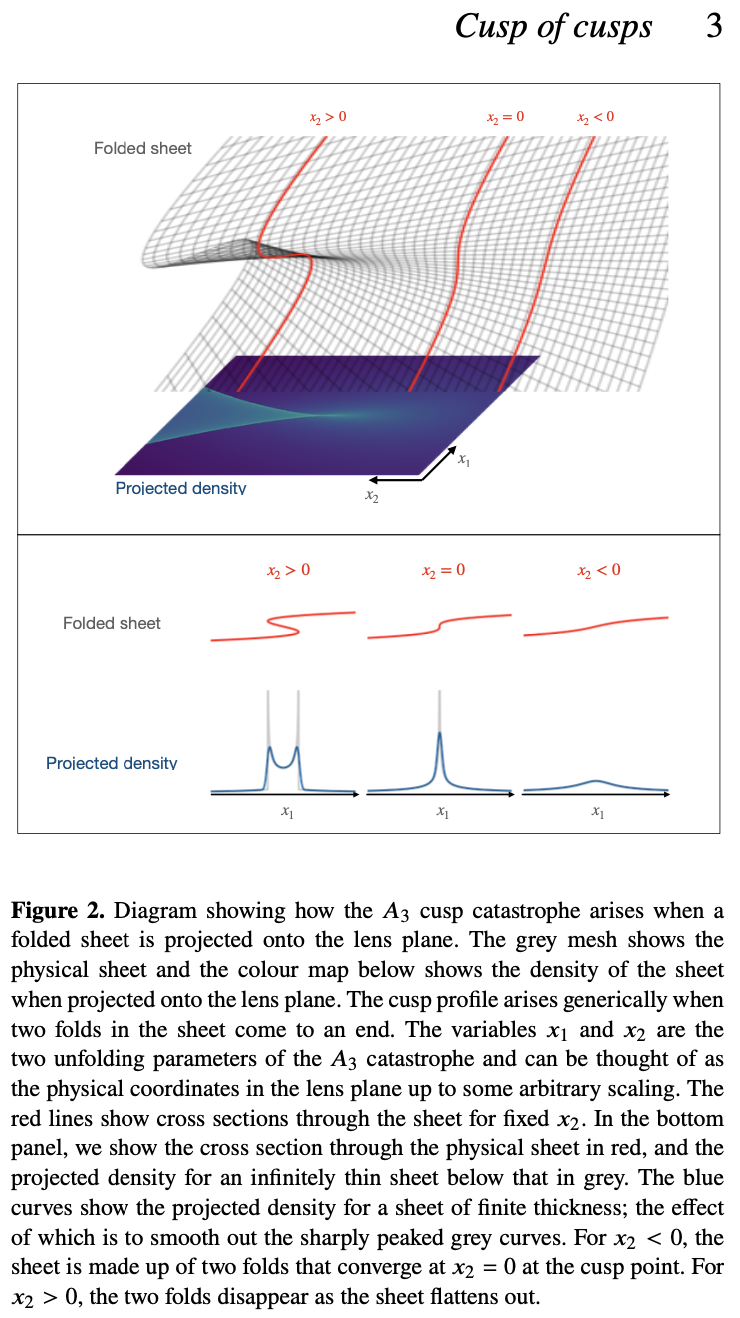
\includegraphics[width=2.85in]{Figures/cusp.png}
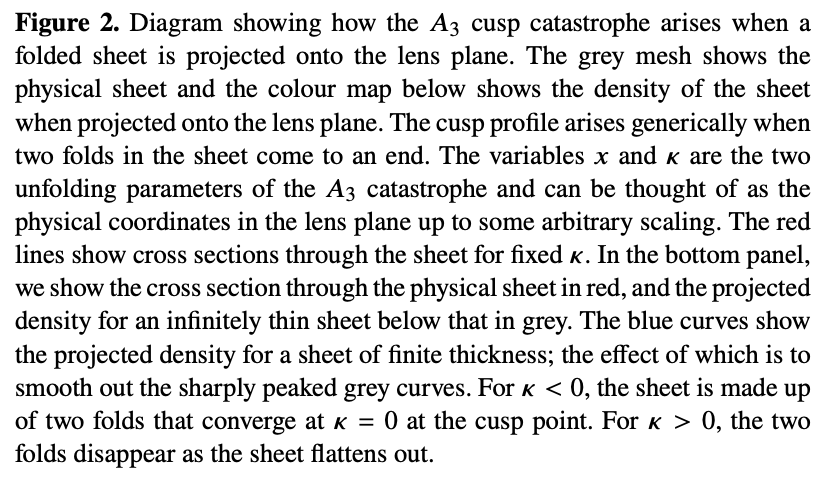
\includegraphics[width=0.5in]{Figures/cuspcaption.png}
Jow+2301.08344
  }

  \frame{
    \frametitle{Extreme Scattering Events}
%\hspace{-0.5in}
\begin{center}
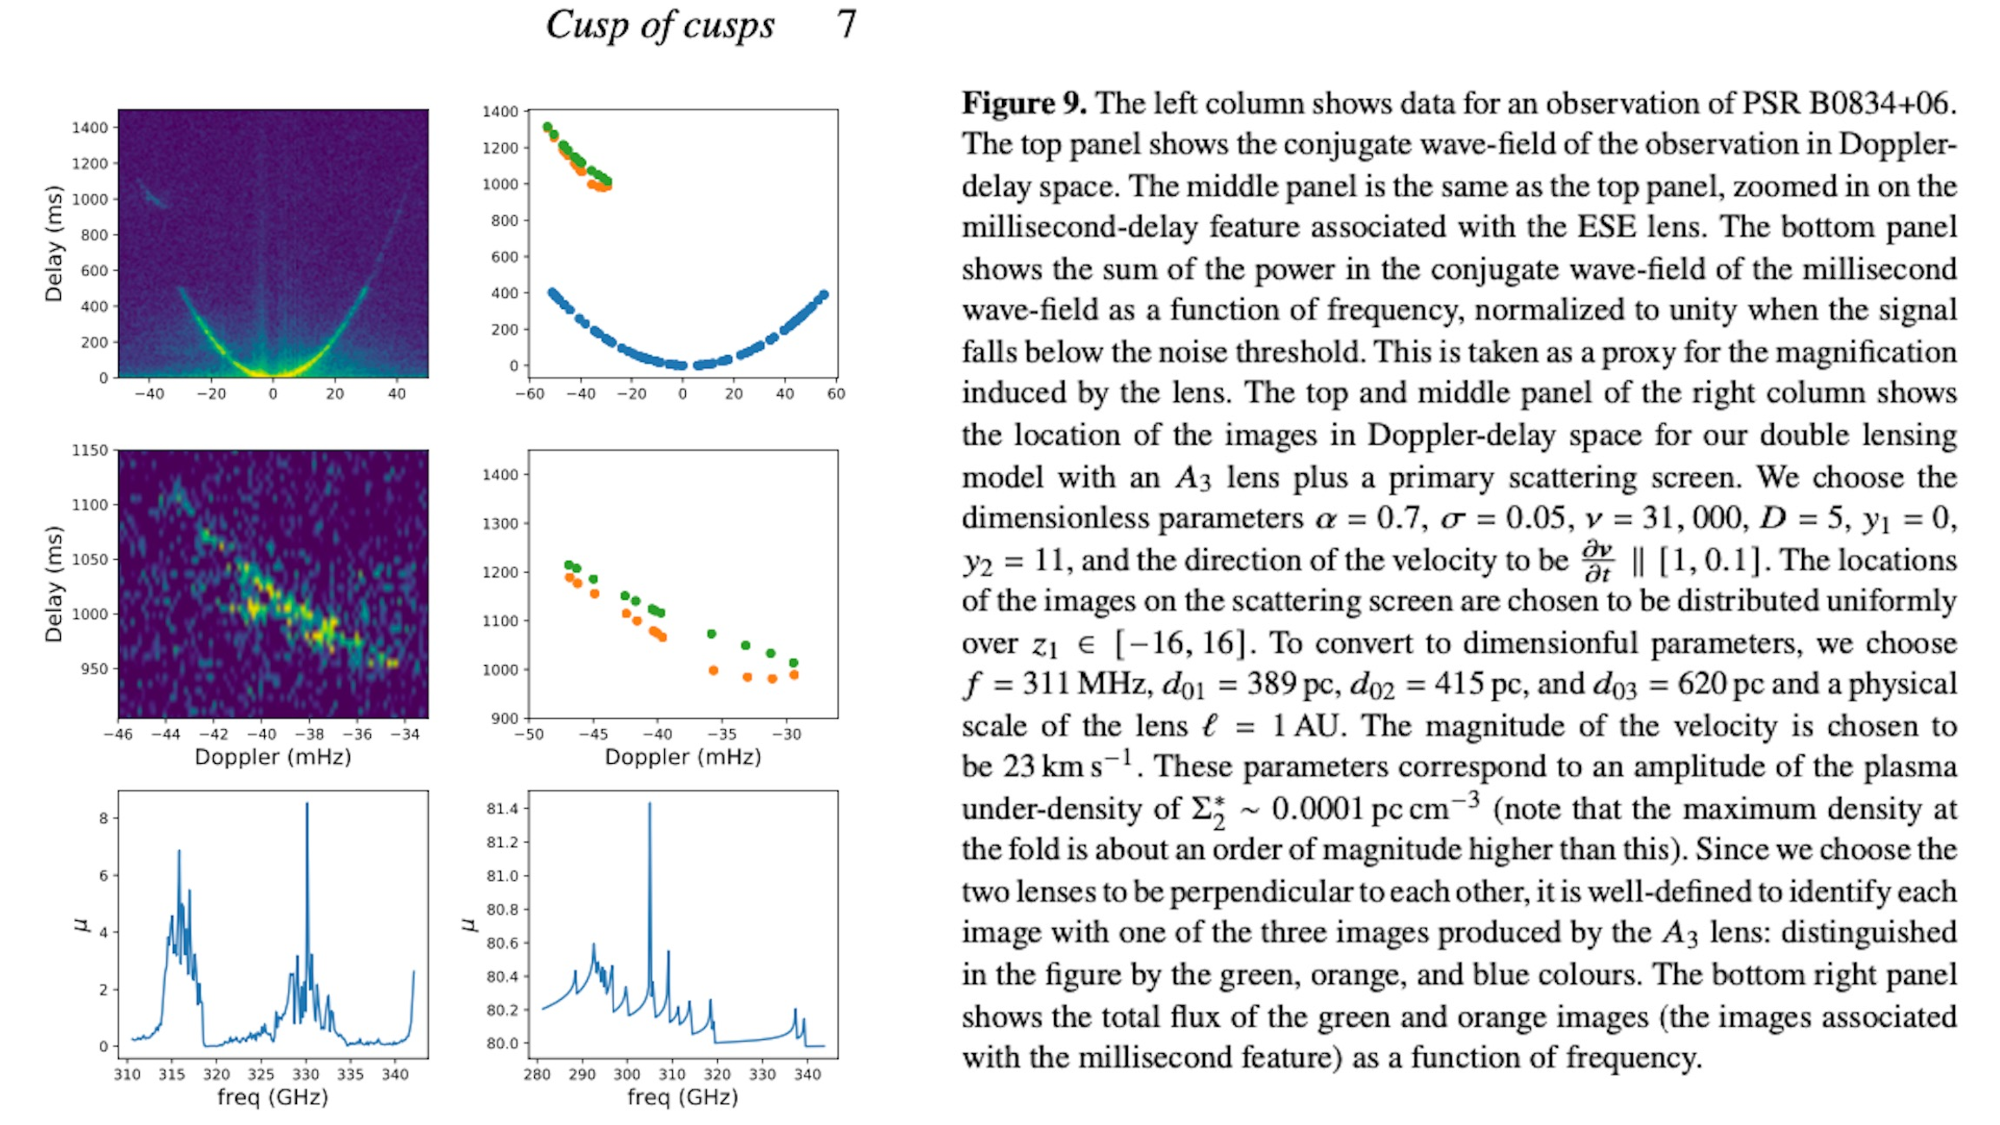
\includegraphics[width=4.65in]{Figures/esemodel.pdf}
\end{center}
  }


  \frame{
\vspace{-0.5in}
    \frametitle{Discussion}
    \begin{itemize}
    \item Eikonal effects applicable to compact radio sources,
      e.g. FRBs, pulsars
    \item full wave
effect dominates for long wavelengths as Fresnel scale is bigger then Einstein radius
    \item microlensing down to planet size
    \item gravitational waves:  LIGO, LISA, PTA
    \end{itemize}
  }




  \frame{
%\vspace{-0.5in}
    \frametitle{Conclusions}
    \begin{itemize}
     \item wave optics changes nature of astrophysical observables: Coherent FRB/pulsar/GW      radiation one of the potentially most
      precise measurements in physics
      \item already makes microarcsecond images of pulsar scattering,
        pico arcsecond of magnetospheres
      \item ISM plasma screens modelled quantitatively as localized
        1-D features, no longer stochastic turbulent volume.
      \item next generation FRB telescopes for cosmic mass inventory,
        possibly dark energy/acceleration
    \end{itemize}
  }

\end{document}
